\begin{table}[H]
    \centering
	\begin{tabular}{lcccc}
	\textbf{Layer Type} & \textbf{Layer Config} & \textbf{Activation}  & \textbf{Output} & \textbf{Params}\\ \hline
	\conv	& \convKSF{5}{3}{5}	& relu		& \texttt{48,86,5} 	& \texttt{380}\\
	\conv	& \convKSF{5}{2}{8}	& relu		& \texttt{24,43,8} 	& \texttt{1008}\\	
	\conv	& \convKSF{3}{1}{12}	& relu		& \texttt{24,43,12} 	& \texttt{876}\\
	\conv	& \convKSF{3}{1}{15}	& relu		& \texttt{24,43,15} 	& \texttt{1635}\\
	\conv	& \convKSF{3}{1}{18}	& relu		& \texttt{24,43,18} 	& \texttt{2448}\\
	
	\flt		& /					& /		& \texttt{20640}		& \texttt{0}\\
	\dns		& \dnsP{64}			& relu		& \texttt{64}		& \texttt{1188928}\\
	\dns		& \dnsP{6}			& softmax	& \texttt{64}		& \texttt{390}\\
	\end{tabular}
	%Total params: 1,195,665
	%Trainable params: 1,195,665
	%Non-trainable params: 0
\end{table}


\begin{table}[H]
	\centering
	\begin{tabular}{lc}
	\textbf{Param} & \textbf{Value}\\ \hline
	Batch Size 	& 32 \\
	Optimizer 	& Adam \\
	Base lr		& 0.001 \\
	\end{tabular}
\end{table}


\begin{figure}[H]
	\begin{center}
	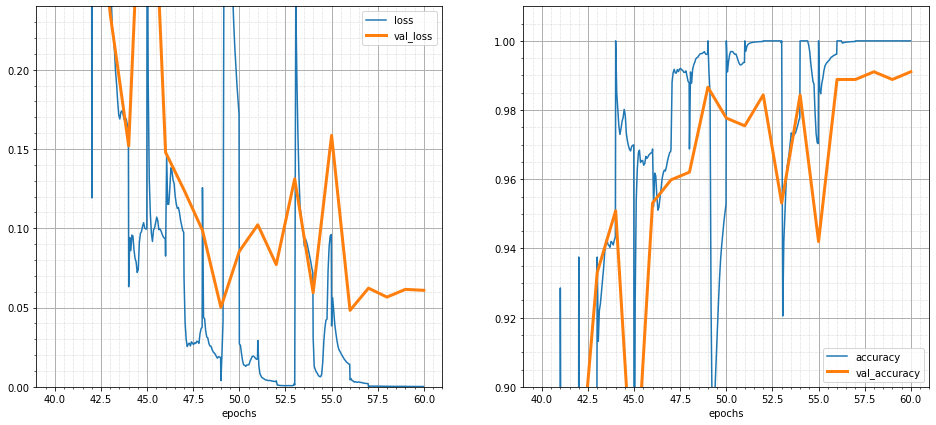
\includegraphics[width=\linewidth]{Immagini/conv-3}
	\caption{Graph of the third run}
	\end{center}
\end{figure}
\begin{table}[H]
	\centering
	\begin{tabular}{cccccc}
		\textbf{Run} &\textbf{Loss}&\textbf{V.Loss} &\textbf{Acc.}&\textbf{V.Acc.}&\textbf{$\Delta$ Acc.} \\ \hline
		1   & 1.0908e-04    &   0.0439  & 1.0000    & 0.9866    & 0.0134 \\
		2   & 8.7761e-05    &   0.0912  & 1.0000    & 0.9888    & 0.0112 \\
		3   & 1.8083e-04    &   0.0609  & 1.0000    & 0.9911    & 0.0089 \\
		\textbf{Avg} & \textbf{1.2589e-04} & \textbf{0.0653}	& \textbf{1.0000}	& \textbf{0.9889} 	& \textbf{0.0112} 
	\end{tabular}
\end{table}

%NOTARE CHE AGGIUNGERE PIU LIVELLI NON AIUTA



